\section{LSST Observing Cadence Optimization to Enhance PHA Completeness \label{sec:opsim}}

LSST takes observations in pairs of visits separated by 20 to 60 minutes. This cadence -- validated in the previous sections -- allows it to increase the sky coverage and improve the survey efficiency relative to taking triplets or quads of visits in each night. There are multiple approaches to covering the sky with pairs of visits. In this section we evaluate the effects of varying the LSST observing strategy and the resulting PHA completeness.

This evaluation is carried out using a combination of the LSST Operations Simulator (OpSim) and the LSST Metrics
Analysis Framework (MAF).
The LSST Metrics Analysis Framework (MAF) is a user-oriented, python package for evaluating the pointing history
from these simulated surveys in light of particular science goals or interests. The various metrics coded in the
MAF framework can be calculated for any given simulated survey and compared as simulation parameters are changed
in OpSim. This permits a thorough investigation of the trades between different observing strategies, in terms of the
effect on multiple science goals, including the PHA completeness.  We first describe the basic steps in our simulations,
then describe the baseline and modified LSST simulated surveys, and then discuss our results.


\subsection{Simulations of LSST Asteroid Discoveries}

The basic components of our end-to-end simulation of asteroid discovery, described in detail below, include
\begin{enumerate}
\item {\it NEO Population Modeling.} Orbital parameters are used to generate asteroid positions during the
simulated survey duration for a simulated or properly debiased extant NEO population. The population needs
to adequately sample color, size and other properties. A database of such positions evaluated with an adequate
time step  is available as an input to MAF.
\item {\it Survey Cadence Modeling.} A series of LSST pointings with instrumental metadata and observing conditions
is generated by OpSim. In addition to boresight positions, the camera orientation and selected filter, available
metadata enable the computation of instrumental sensitivity (limiting magnitudes).
\item {\it Asteroid Optical Flux Modeling.}  Optical flux from an arbitrary asteroid needs to be computed
as a function of the positions of the Sun, the asteroid and Earth, and asteroid physical properties (e.g., size
and color). This model is implemented in MAF.
\item {\it Source Detection Modeling.} Given the instrument model, observing conditions and asteroid flux,
the signal-to-noise ratio is estimated and used to compute detection probability. This model is implemented
in MAF.
\item {\it Detection Linking Modeling.}  Instead of running MOPS, a model that emulates MOPS
performance is used to significantly speed up the computations. This is equivalent to assuming that an object is discovered 
if a given pattern of observations for an object is achieved. This model is implemented
in MAF.
\item {\it Completeness Estimation.} Given a list of ``discovered objects'', and the input population,
the completeness is estimated as a function of asteroid properties (e.g. size) and various other parameters
(e.g. observing strategy). This model is implemented in MAF.
\end{enumerate}

We proceed to describe these models in more detail, and then discuss the baseline and several modified LSST
surveys, and the corresponding PHA completeness estimates.

\subsubsection{NEO Population Modeling \label{sec:MAFdetails}}

We use random samples from the synthetic solar system model (S3M) presented in \cite{Grav2011} in order to model completeness for NEOs and PHAs. We have chosen a sample of 2000 NEOs from the \cite{Grav2011} NEO population, which is based on the \cite{Bottke2002} model. We chose a separate sample of 2000 PHAs from the same model, by choosing NEOs with a MOID $\le 0.05$~AU. The PHA population is useful for evaluating PHA completeness directly; the NEO population is useful for comparison to other survey evaluations. A plot of the $a$, $e$, $i$ distributions for these PHAs and NEOs is shown in Figure~\ref{fig:PHA_orbits}.

With this small set of orbits, we then assume that the $H$ magnitude distribution is independent of the orbital distribution.
 For most small body populations, including the PHA population larger than 140~m in diameter, this is approximately true. 
 Assuming an independent distribution, each orbit can be ``cloned'' from the fiducial $H$ magnitude to a range of values 
 covering the interesting sizes for analysis; this allows the analysis to use a large number of objects at each $H$ value, without 
 requiring extensive resources to generate ephemerides for a much larger set of orbits. We use the small population of 
 2000 NEOs or PHAs and clone them to a range of $H$ magnitudes between $H$=14 and $H$=28, with bins of 0.2 in $H$,
 using $dN/dH = 10^{\alpha\, H}$, with $\alpha=0.33$ \citep{2017Icar..284..114S}. We have verified with a larger simulated set 
 of NEOs that reducing the population to 2000 NEOs does not significantly alter the completeness calculation.

Using the details of the input population, MAF generates the expected observations of each object using the pointing history
from a specific OpSim simulated survey. Ephemerides are generated using OpenOrb \citep{OpenOrb2009} for a closely spaced grid of times (typically every 2 hours), and then interpolated to the exact times of each OpSim pointing.


\begin{figure}[t!]
\centering
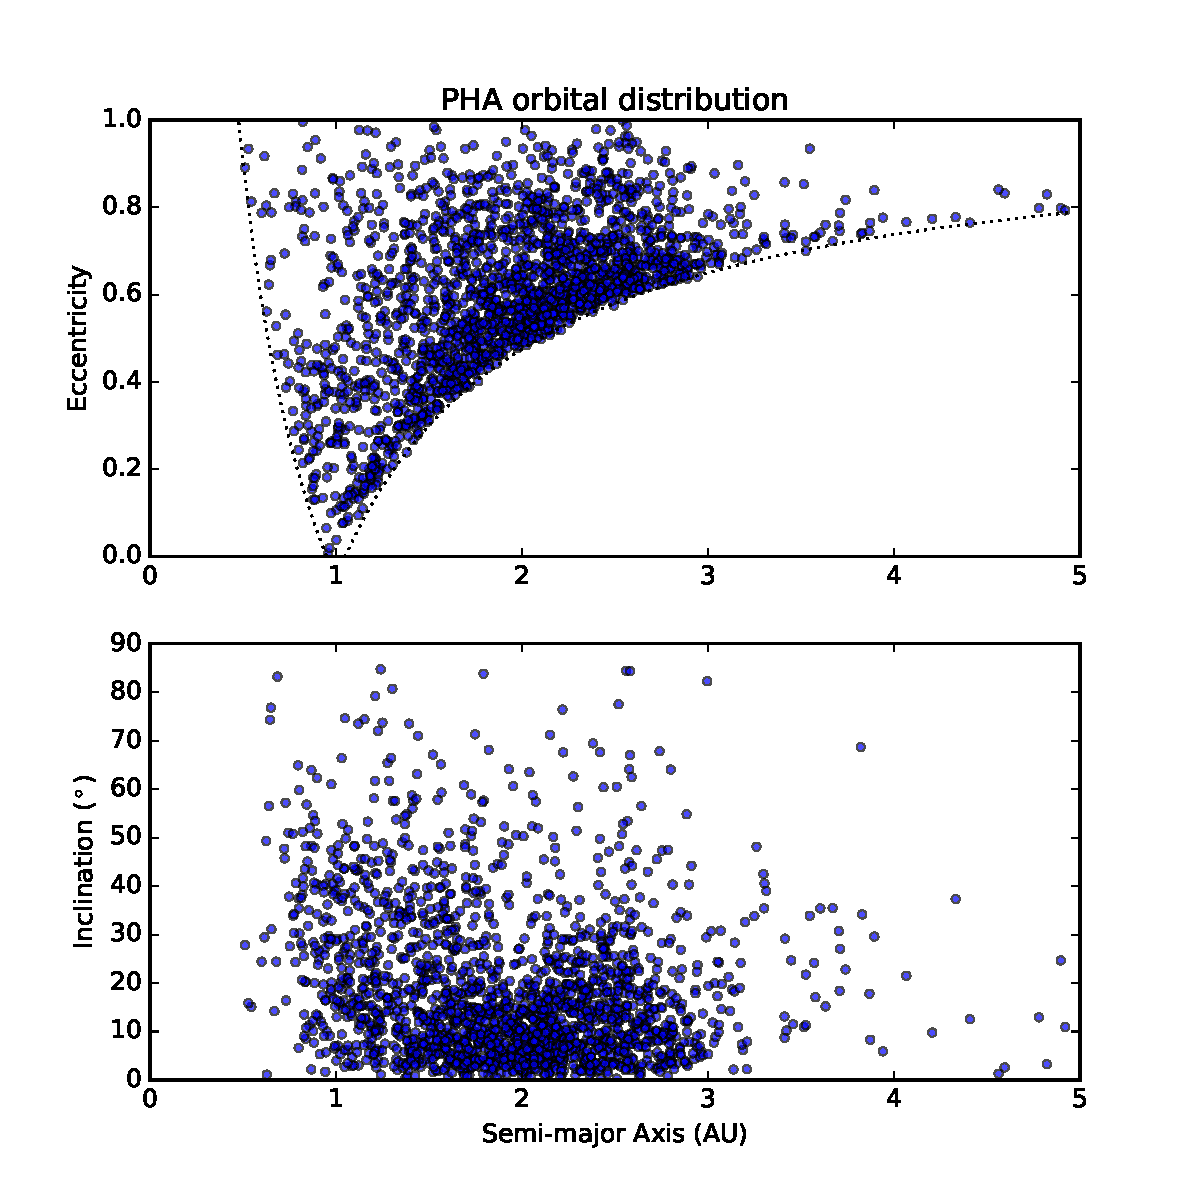
\includegraphics[width=0.49\textwidth]{figures/phas_2k_orbits}
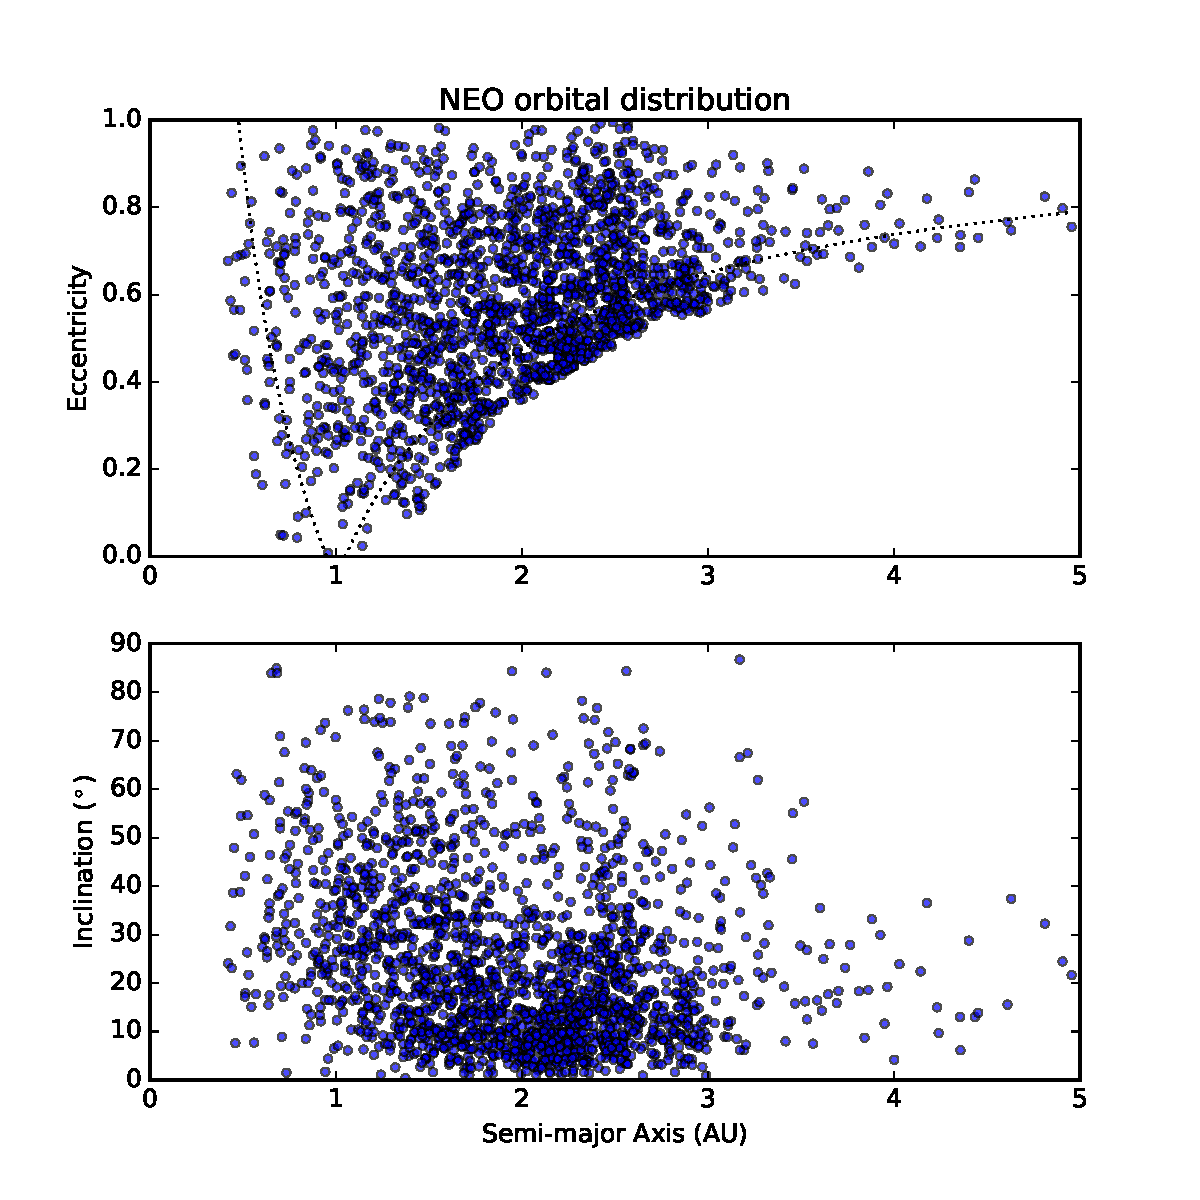
\includegraphics[width=0.49\textwidth]{figures/neos_2k_orbits}
\vskip -0.2in
\caption{The eccentricity and inclination distributions, as a function of semi-major axis, of the PHAs (left) and NEOs (right) used in this analysis. Both populations were randomly sampled from the S3M model \citep{Grav2011}, a synthetic solar system model based on the \cite{Bottke2002} NEO orbital distribution. NEOs are defined as objects with $q<1.3$~AU; PHAs are defined as having a Minimum Orbit Intersection Distance (MOID) with Earth of less than 0.05~AU (implying $q\le1.05$~AU) and having $H\le22$.  The dotted lines correspond to q = 1.05~AU and Q = 0.95~AU, the approximate limits where MOID$\le 0.05$~AU. \label{fig:PHA_orbits}}
\end{figure}

\subsubsection{Survey Cadence Modeling}

The LSST Operations Simulation \citep[OpSim,][]{delgado14} is a Python software package that generates a realistic pointing history, with the time, filter, location, astronomical conditions, weather conditions, and predicted point-source $5\sigma$ limiting magnitude, for each LSST visit
over the lifetime of the survey. This pointing history is generated using weather data (cloudiness and seeing) from the Cerro Pach\'{o}n site and a high-fidelity model of the telescope itself (including slew and settle time and dome movement, for example), combined with a parameterized set of observing proposals that determine how the scheduling algorithm attempts to gather observations. By configuring OpSim with different parameters for the observing proposals, we can generate a series of simulated surveys which prioritize different science goals. The LSST baseline survey and its modifications designed to enhance the PHA completeness are described in detail
in \S\ref{sec:surveys} below.


\subsubsection{Asteroid Optical Flux Modeling}

Given $H$ magnitude for an object, its apparent magnitude in Johnson's $V$ band can be easily computed
given the positions of the object, the Sun and the observer; we have used the two-parameter H-G magnitude 
system \citep{1989aste.conf...21B}, assuming G=0.15.
Magnitudes, or fluxes, in any other optical and near-IR band (in case of LSST, $u$, $g$, $r$, $i$, $z$, and $y$)
can be computed from $V$ magnitude by specifying a spectrum for each object. We have
assumed that our entire NEO population has the same spectral energy distribution as C-type main-belt asteroids.
The computed color transformations for LSST bandpasses are listed in Table~\ref{tab:sed_colors}. Choosing the
spectral energy distribution of  S-type main-belt asteroids instead results in $<$1\% changes in completeness.
These simulation-based colors were verified using SDSS observations \citep{2001AJ....122.2749I} and analogous
computations with SDSS bandpasses.

\begin{deluxetable}{ccccccc}
\centering
\tablecolumns{7}
\tablecaption{Color transformations from Johnson's $V$ band to LSST bandpasses, for C and S type asteroids. \label{tab:sed_colors}}
\tablewidth{0.7\textwidth}
\tablehead{ Type & $V-u$ & $V-g$ & $V-r$ & $V-i$ & $V-z$ & $V-y$  \\ }
\startdata
C  & -1.53 &  -0.28 &  0.18 &  0.29 &  0.30 & 0.30 \\
S & -1.82 &  -0.37 &  0.26 & 0.46 &  0.40 & 0.41  \\
\enddata
\end{deluxetable}


\subsubsection{Source Detection Modeling}


\begin{figure}[t!]
\centering
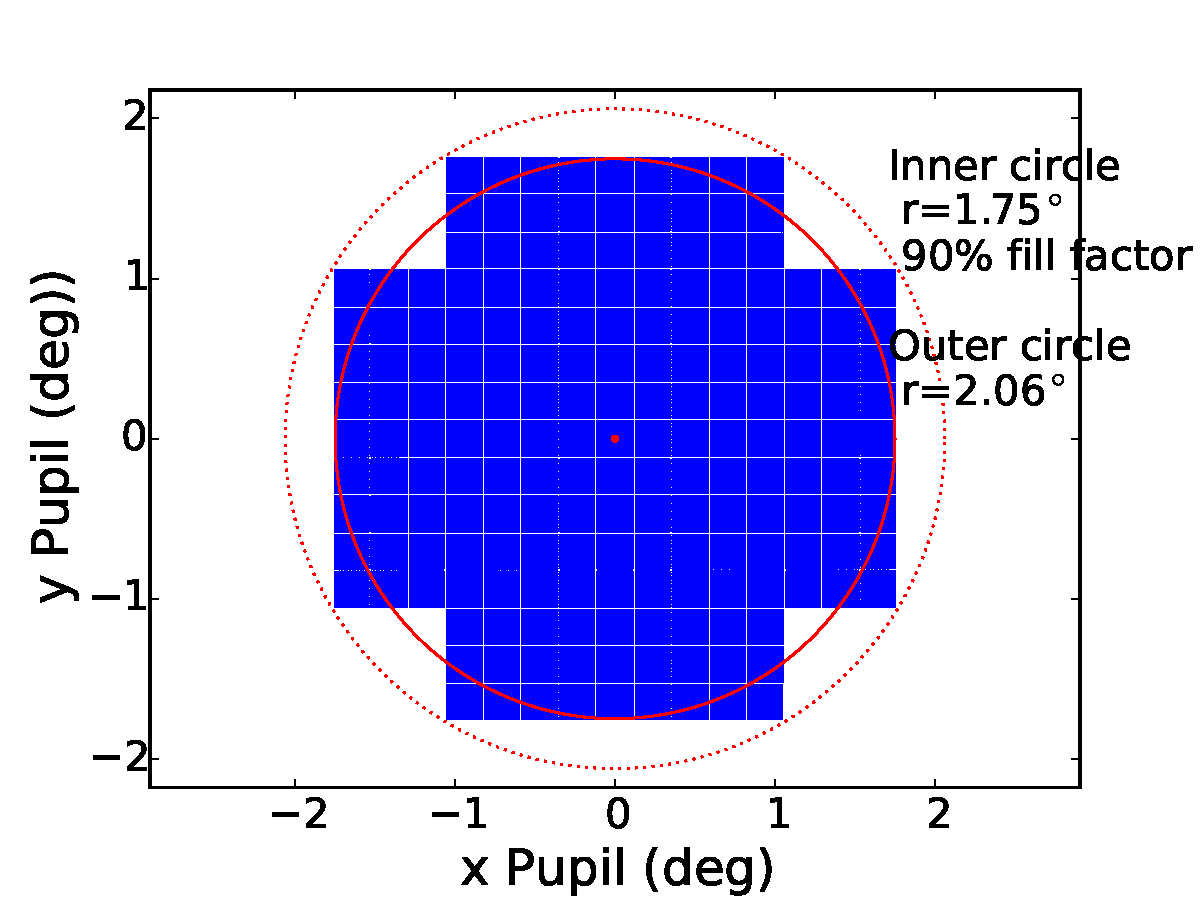
\includegraphics[width=0.65\textwidth]{figures/focalplane}
\caption{Model of the LSST camera footprint, including chipgaps and CCD + raft layout. \label{fig:camera_footprint}}
\end{figure}

If the object is within the LSST field of view, its predicted position, velocity, and apparent $V$ magnitude (calculated from the fiducial $H$ magnitude associated with the orbit) is recorded along with information about the simulated observation itself (such as the seeing, limiting magnitude, filter, and boresight RA/Dec). The full LSST camera footprint (see Figure~\ref{fig:camera_footprint}), including chip gaps, is
used to determine whether an object is within the field of view.

MAF also calculates signal-to-noise (SNR) loss due to trailing for each observation, which is required when evaluating whether
a particular object is detectable in a given observation. Trailing losses occur whenever the movement of an object spreads its photons over a wider area than a simple stellar point spread function (PSF). There are two aspects of trailing loss to consider: SNR losses and detection algorithm losses. The first is the
irreversible degradation in SNR that occurs because the trailed object includes a larger number of background pixels in its footprint, compared to a stationary PSF. The second effect, detection loss, occurs because source detection software is optimized for detecting point sources; a stellar PSF-like matched filter is used when identifying sources that pass above the defined threshold. This filter is non-optimal for trailed objects but losses can be mitigated with improved software ({\it e.g.} detecting to a lower PSF-based SNR threshold and then using a variety of trailed PSF filters to detect sources). When considering whether a source would be detected at a given SNR using typical source detection software, the sum of SNR trailing and detection losses should be used. With an improved
algorithm optimized for trailed sources (implying additional scope for LSST data management), the smaller SNR losses should be
used instead.

\begin{figure}[t!]
\centering
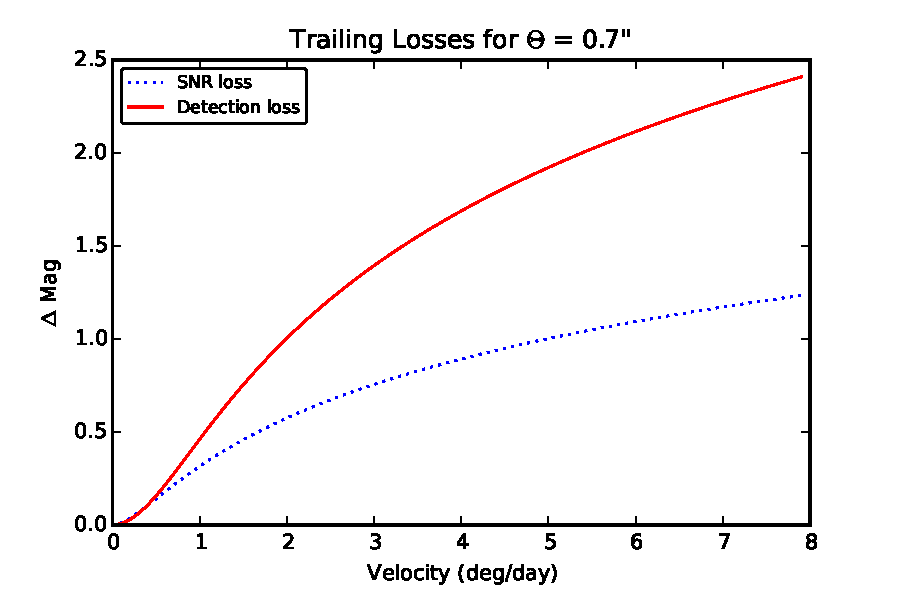
\includegraphics[width=0.85\textwidth]{figures/trailing_losses}
\caption{Trailing losses for 30 second LSST visits, assuming seeing of
  0.7''. The dotted line shows SNR trailing losses, the solid line
  indicates cumulative losses that also account for non-optimal detection
  algorithm. With software improvements the latter detection losses can be
  mitigated. At the fiducial $v=1$ deg/day, the SNR loss is $\sim$0.3 mag,
  and non-optimal detection algorithm contributes an additional loss of
  $\sim$0.16 mag.
\label{fig:trailinglosses}}
\end{figure}

Our simulations of these effects show that both types of trailing losses can be fit well with the
same functional form:
\begin{eqnarray}
\Delta \, m & = &-1.25 \, log_{10} \left( 1 + \frac{a \, x^2} { 1 + b\,
    x} \right) \\
x & = & \frac{v \, T_{exp}} {24 \, \theta}
\end{eqnarray}
where $v$ is the velocity (in deg/day), $T_{exp}$ is the exposure time (in seconds), and $\theta$ is the FWHM (in arcseconds). For trailing SNR losses, we find $a = 0.67$ and $b = 1.16$; for the cumulative loss, that includes both SNR and detection losses,
we find $a=0.42$ and $b=0$. An illustration of the magnitude of these trailing loss effects for 0.7 arcsec seeing is given in Figure~\ref{fig:trailinglosses}.

We calculate the probability of detecting a particular source given its magnitude $m$
and the $5\sigma$ limiting magnitude $m_5$ (after accounting for trailing losses) using a logistic function
\begin{eqnarray}
     P & = & \left[ 1 +  {\rm exp}\left(\frac {m -  m_5}{\sigma}\right) \right]^{-1}.
\end{eqnarray}
where $\sigma$=0.12 describes the width of the completeness falloff \citep{2014ApJ...794..120A}. A source is randomly classified
as detected using the probability $P$. We also evaluate more optimistic discovery criteria using only SNR trailing losses
(i.e. without taking detection losses into account), as well as detections to SNR=4 instead of SNR=5.  This detection model assumes a flat $m_5$
value across the focal plane; no vignetting or background variation (or masking) due to bright stars is included. These effects however are small.


\subsubsection{Detection Linking Modeling}

Once we have computed the set of all visits in which a given object was within the field of view and detected, we locate subsets of these visits that match our target discovery criteria. These criteria generally consist of a given number of visits within a specified
time span within a single night, followed by a given number of additional nights (each with the same required number
of visits in the same time span) falling within a specified time window. The basic criteria is a pair of visits in each
night occurring within 60 minutes, repeated for 3 nights within a 15 day time window. However, we also evaluate
the effect of varying the discovery criteria to require triplets or quads of visits within a single night, and increase
the length of the search window from 15 to 30 days. 

\subsubsection{Completeness Estimation}

With each unique set of discovery criteria, we have a record of what objects would be ``discovered'' at each $H$ value.
With this we calculate the differential discovery completeness, the fraction of objects discovered at a given $H$ magnitude.
To turn this into a cumulative discovery completeness, we simply integrate over $H$, assuming a given $H$ distribution
for the population (recall that we use $dN/dH = 10^{\alpha\, H}$, with $\alpha$ = 0.33).


\subsection{The LSST Baseline Survey\label{sec:surveys}}

The current baseline observing strategy for LSST is represented by our reference run, minion\_1016. This simulated survey
contains observations balanced between several different observing proposals as follows:
\begin{enumerate}
\item The Wide, Fast, Deep (WFD) proposal (also known as the Universal proposal) is the primary LSST survey, expected to receive about 90\% of the observing time and to cover 18,000 deg$^2$ of sky. In the baseline observing strategy, this proposal is configured to obtain visits in pairs spaced about 30 minutes apart, and will typically return to each field about every 3-4 days, balancing the six $ugrizy$ filters. The footprint for the WFD proposal covers approximately $+5^\circ$ to $-60^\circ$ in declination, with a full range of RA values except for a region around the Galactic plane. This declination range corresponds to an airmass limit of about 1.3 when the fields are at an Hour Angle of $\pm$2 hours. In minion\_1016, the WFD proposal receives 85\% (2,083,758) of the total number of visits.
\item The North Ecliptic Spur (NES) proposal is an extension to the WFD to reach the northern limits of the Ecliptic plane ($+$10 degrees), and allows higher airmass observations. The visit timing is similar to the WFD, although the $u$ and $y$ filter are not requested in this region. In the baseline observing strategy, minion\_1016, each NES field requests about 40\% of the total number of WFD visits per field when considering $griz$ filters only (304 visits per field in $griz$ vs 795 visits per field in $griz$ in WFD), and receives 6\% (158,912) of the total number of visits.
\item The Deep Drilling Fields (DD) proposal includes a set of single pointings that are requested in extended sequences; currently these sequences are $grizy$ visits, with additional coverage in $u$ band. Each sequence requires about an hour of observing time, and is repeated every few days. In minion\_1016, there are 5 DD fields, 4 of which correspond to fields which have been officially selected
by the Project and announced to the community; these five fields receive 5\% of the total visits.
\item The Galactic Plane (GP) proposal covers the region with high stellar density around the Galactic plane not covered by the WFD. This proposal requests a small number of visits in each of the six $ugrizy$ filters, with no timing constraints. In minion\_1016, this proposal receives 2\% of the total visits.
\item The South Celestial Pole (SCP) proposal is an extension of the WFD footprint to cover the region south of $-60^\circ$ declination. Like the GP, this proposal requests a small number of visits in each of the six $ugrizy$ filters, with no timing constraints. In minion\_1016, this proposal receives 2\% of the total visits.
\end{enumerate}

This is summarized in Table~\ref{tab:surveysummary}. The footprint of these various proposals in the baseline minion\_1016 reference run is shown in Figure~\ref{fig:minion_footprints}. In each proposal, the individual visits are 30 seconds long, consisting of two back-to-back coadded 15 second exposures.

\begin{deluxetable}{lccccc}
\tablecaption{Summary of the proposals in the baseline minion\_1016 simulated survey. \label{tab:surveysummary}}
\tablehead{Proposal & Filters & Pairs? & Number of fields & Number of visits/field & \% total visits}
\startdata
Wide Fast Deep & $ugrizy$ & Yes & 2293 & 908 & 85 \\
North Ecliptic Spur & $griz$ & Yes & 521 & 344 & 6 \\
Deep Drilling & $ugrizy$ & Yes & 5 & ~23,000 & 5 \\
Galactic Plane & $ugrizy$ & No & 230 & 180 & 2 \\
South Celestial Pole & $ugrizy$ & No & 293 & 180 & 2 \\
\enddata
\end{deluxetable}


\begin{figure}[t!]
\centering
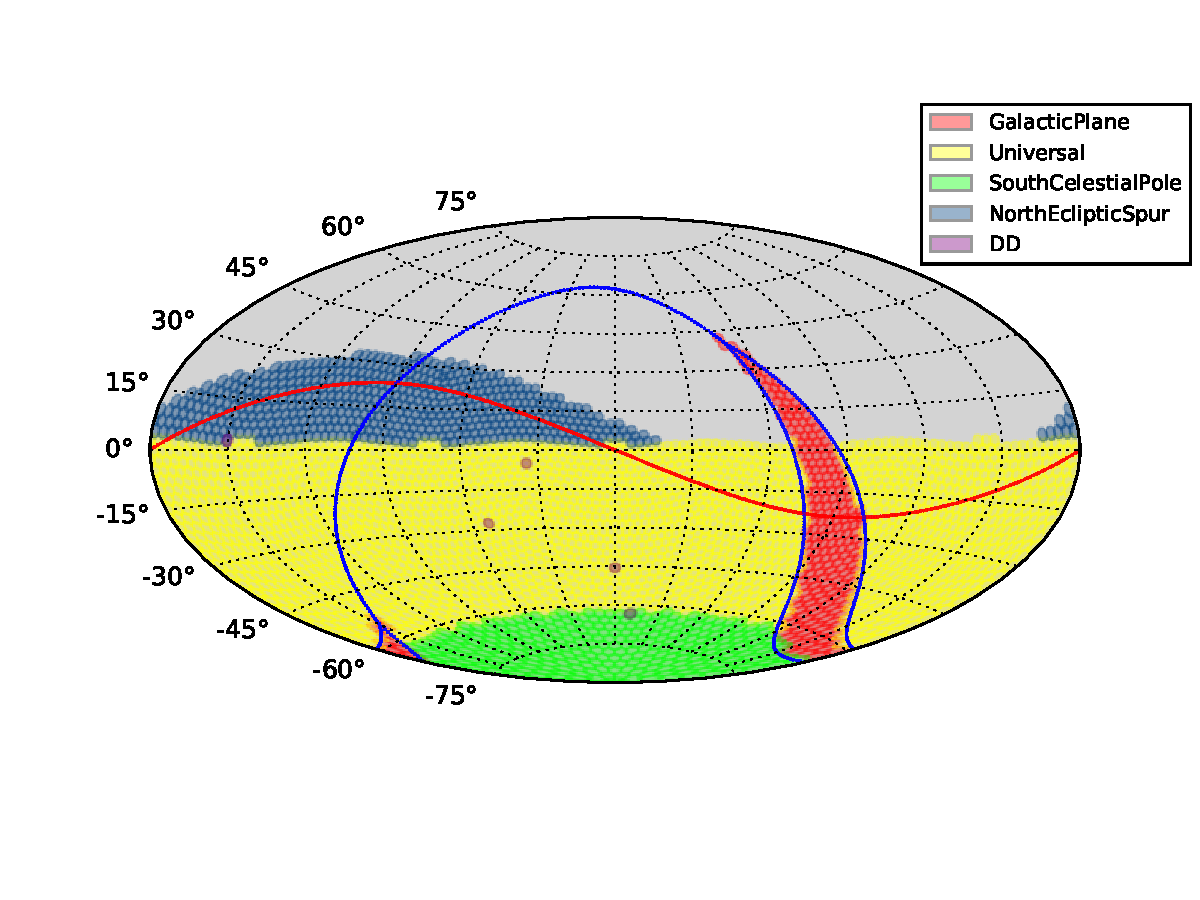
\includegraphics[width=0.85\textwidth]{figures/minion_1016_proposal_footprint}
\vskip -1.0in
\caption{The footprints of the various proposals included in the baseline observing strategy, represented by reference run minion\_1016. In the reference run, the WFD proposal receives 85\% of the total visits, the NES receives about 6\% of the
total visits, the DD receives about 5\% of the total visits, and the GP and SCP each receive about 2\% of the total visits. 
In the baseline run, every visit is 30s long, consisting of two back-to-back 15s exposures.
\label{fig:minion_footprints}}
\end{figure}


\subsection{Baseline Survey Discovery Completeness}

Using the baseline survey run, minion\_1016, with the baseline discovery
criteria (pairs of visits occurring within 60 minutes and
repeated for 3 nights within a 15 day time window), we find a cumulative
completeness of
\begin{equation}
C_{\rm PHA, baseline}(H\le22) = 65.6\%
\end{equation}
at $H\le22$ for our PHA input population. This is LSST's baseline expected PHA completeness, derived using the reference cadence and the design MOPS and data management requirements. The cumulative completeness as a function of $H$ magnitude is shown in Figure~\ref{fig:minionC1}). 

When an NEO population is used instead of a PHA input population, the cumulative completeness is:
\begin{equation}
C_{\rm NEO, baseline}(H\le22) = 60.7\%
\end{equation}
or about 5\% lower than for the PHAs
(see also Figure~\ref{fig:minionC1}). This is primarily due to differences in the orbital distribution differences, as illustrated in Figure~\ref{fig:PHA_orbits}. The definition of PHAs includes a Minimum Orbit Intersection Distance (MOID) with Earth of 0.05~AU, requiring PHAs to more closely approach Earth than NEOs (which are defined as simply having $q<1.3$~AU), and thus the PHAs achieve brighter peak V magnitudes than the NEOs. To quantify this effect, we calculated the apparent $V$ magnitude for both the NEO and PHA input populations every night for ten years, while accounting for trailing losses and assuming a constant $H=22$ magnitude for every member of the population. The resulting mean value of the
brightest 10-year $V$ magnitudes are about half a magnitude brighter for PHAs than for NEOs.

Note that all the completeness results presented in this section assume that no objects are known prior to LSST survey, and thus are lower than estimates including other surveys. We'll return to the impact of adding discoveries by the  rest of the NEO discovery system in \S\ref{sec:known}. 

\begin{figure}[t!]
\centering
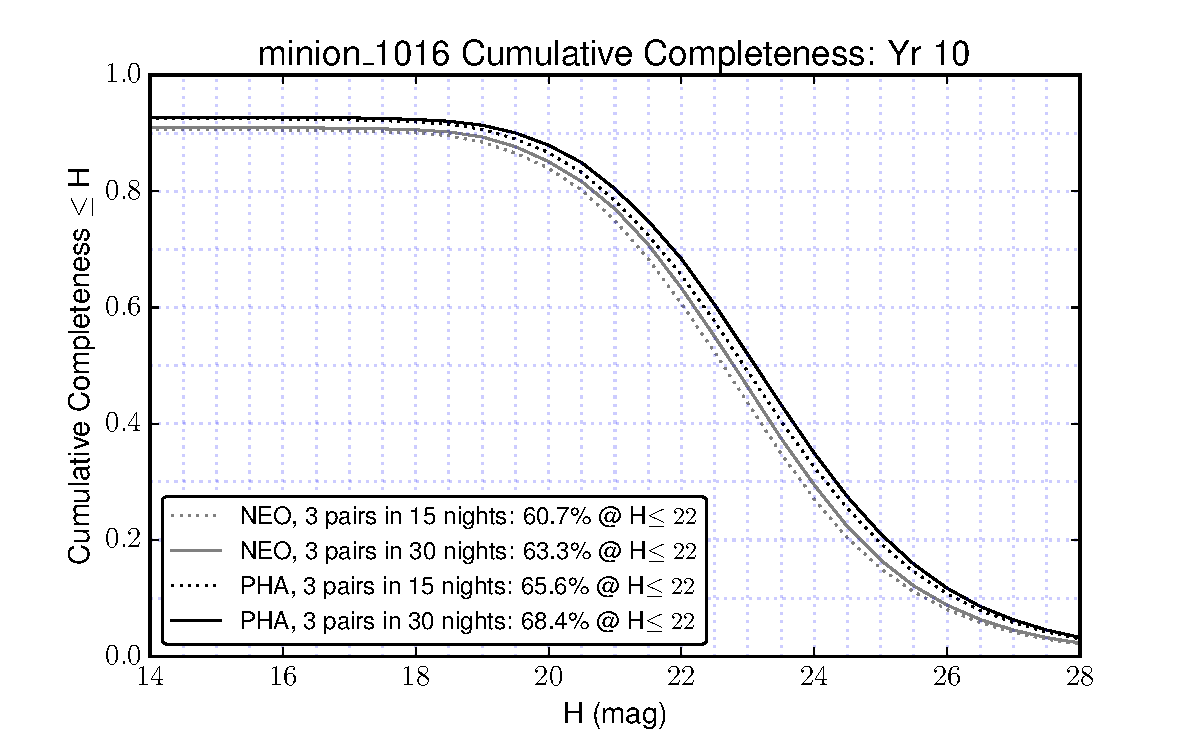
\includegraphics[width=0.99\textwidth]{figures/minion_1016_NEO_and_PHA_Cumulative_Completeness}
\vskip -0.2in
\caption{The cumulative completeness for PHAs and NEOs, as a function of absolute magnitude $H$, for the baseline
cadence minion\_1016. The completeness is below 100\% at the bright end (large size limit) because some objects have
synodic periods longer than the survey duration (and thus effectively ``hide'' behind the Sun), and some are visible but
 do not receive the required number of observations due to telescope scheduling. \label{fig:minionC1}}
\end{figure}

\begin{deluxetable}{lccccccc}
\tablecaption{The cumulative completeness for PHAs with $H\le22$ for various
survey strategies (rows) and MOPS discovery criteria (columns). The numbers presented here are for LSST alone, and do not include discoveries made by other surveys. In addition to changing the overall duration of the survey (12 years instead of 10), the
completeness is shown for different track linking windows ($N_w=15$ or $30$ days),
enhanced detection algorithms to reduce trailing losses (``Trail Det''), and
lowering the individual detection threshold from SNR$=5$ to SNR$=4$. These columns therefore map to software or computational capability enhancements, while the rows map to different survey cadences. See the text for detailed description of individual survey strategies. \label{tab:completeness}}
\tablehead{
                   & \multicolumn{3}{c}{10 year survey}  &  \multicolumn{4}{c}{12 year survey}  \\
    \cmidrule(r){2-4} \cmidrule(r){5-8}
Simulation  & $N_w$=15 & $N_w$=30 & $N_w$=30 & $N_w$=15 & $N_w$=30 & $N_w$=30 & $N_w$=30 \\
                   &                   &                    & Trail Det     &                   &                   &  Trail Det    &  SNR=4 
}
\startdata
LSST baseline & 65.6 & 68.4 & 69.1 &  --- & --- & --- & --- \\
Extra ecliptic visits & 66.1 & 69.8 & 70.5 & 70.5 & 73.9 & 74.8 & 77.1 \\
Longer ecliptic visits & 63.2 & 67.5 & 70.5 & 67.3 & 71.7 & 74.5 & 75.7 \\
NEO-focused cadence & 66.5 & 70.3 & 72.3 & 70.2 & 73.8 & 75.8 & 77.2 \\
\enddata
\end{deluxetable}


\subsection{Enhancing the Discovery Yields}

Given the baseline presented above, we can examine the effects of changing both the survey design (reallocating telescope resources) and improving the software and/or devoting more computing resources to the linking problem.

% There is an interplay between adjusting software requirements and survey strategy -- as an obvious example, software requiring triplets of visits per night instead of pairs will result in much different completeness results if the survey was designed to only request two visits per night rather than three. Likewise, some changes in survey design work best with changes to the algorithms or discovery criteria; for example, lengthening the visit time increases the detection losses and pushing source detection to the ``trailing loss'' limit is required for a significant improvement in completeness. We compare possible improvements to software within a single simulated survey as much as possible, there are some algorithmic options which require surveys using different observing strategies for a meaningful comparison.

\subsubsection{Enhancing the Discovery Yields: Software}

The baseline analysis assumed that only objects linked in 15 day ``windows'' will be discovered, consistent with the design requirements and measured performance of LSST's implementation of MOPS. It is instructive to examine how much better the LSST would perform if further investment is made in enhancing the LSST software system (primarily MOPS, but image differencing as well).

Continuing to use the baseline minion\_1016 simulation, we explore the impact of possible software improvements on discovery rates. The results are detailed in Table~\ref{tab:completeness}. We find:

\begin{itemize}
\item {\bf 30-day window}: Extending the MOPS window for linking pairs of detections from the nominal 15 day window to a 30 day window increases completeness by about 3\%. This change also comes with an increase in computational requirements by about an order of magnitude (see Appendix \ref{sec:appMOPS}).

\item {\bf Detecting trailed sources}: Enhancing source detection algorithms to detect trailed $SNR=5$ objects increased completeness by about 0.5\% relative to the baseline, with little sensitivity to linking window size. This is because for most PHAs (and NEOs) LSST gets multiple discovery opportunities over the 10yr survey period.

\item {\bf Detecting at SNR=4}: Using sources detected down to SNR=4 instead of SNR=5 increases completeness by about 3.5\% relative to baseline. However, the change also leads to an estimated increase in the compute requirements by about two orders of magnitude (see \S\ref{sec:kaiser}).

\end{itemize}

Widening the MOPS tracklet linking window from 15 to 30 days achieves a meaningful gain in completeness relative to the baseline, with a reasonable marginal computational cost (discussed in \S\ref{sec:discussion}). The increased window allows more opportunities to capture a set of observations which meet the MOPS discovery criteria.

We also note that the current OpSim behavior does not prioritize capturing large chunks of contiguous sky, often leaving gaps in coverage from night to night. Therefore, with the large LSST field of view, after 30 days the areal coverage will be much more evenly distributed than after 15 days enhancing the 30-day-window yields.
Changes to the scheduling algorithm to favor covering contiguous blocks of sky\footnote{A similar modification of
the baseline cadence, the so-called ``rolling cadence'', is also favored by the supernovae science programs. A release of a series of simulated surveys implementing this idea is anticipated for late 2017.} are likely to further improve the completeness.

The upper limit to yield improvements due to software enhancements is likely $\gtrsim 10$\%; this is illustrated in Figure~\ref{fig:more_completeness}, where requiring only a single night of pairs or requiring 6 observations in any sequence over 60 nights increases completeness over 10\%.


\begin{figure}[t!]
\centering
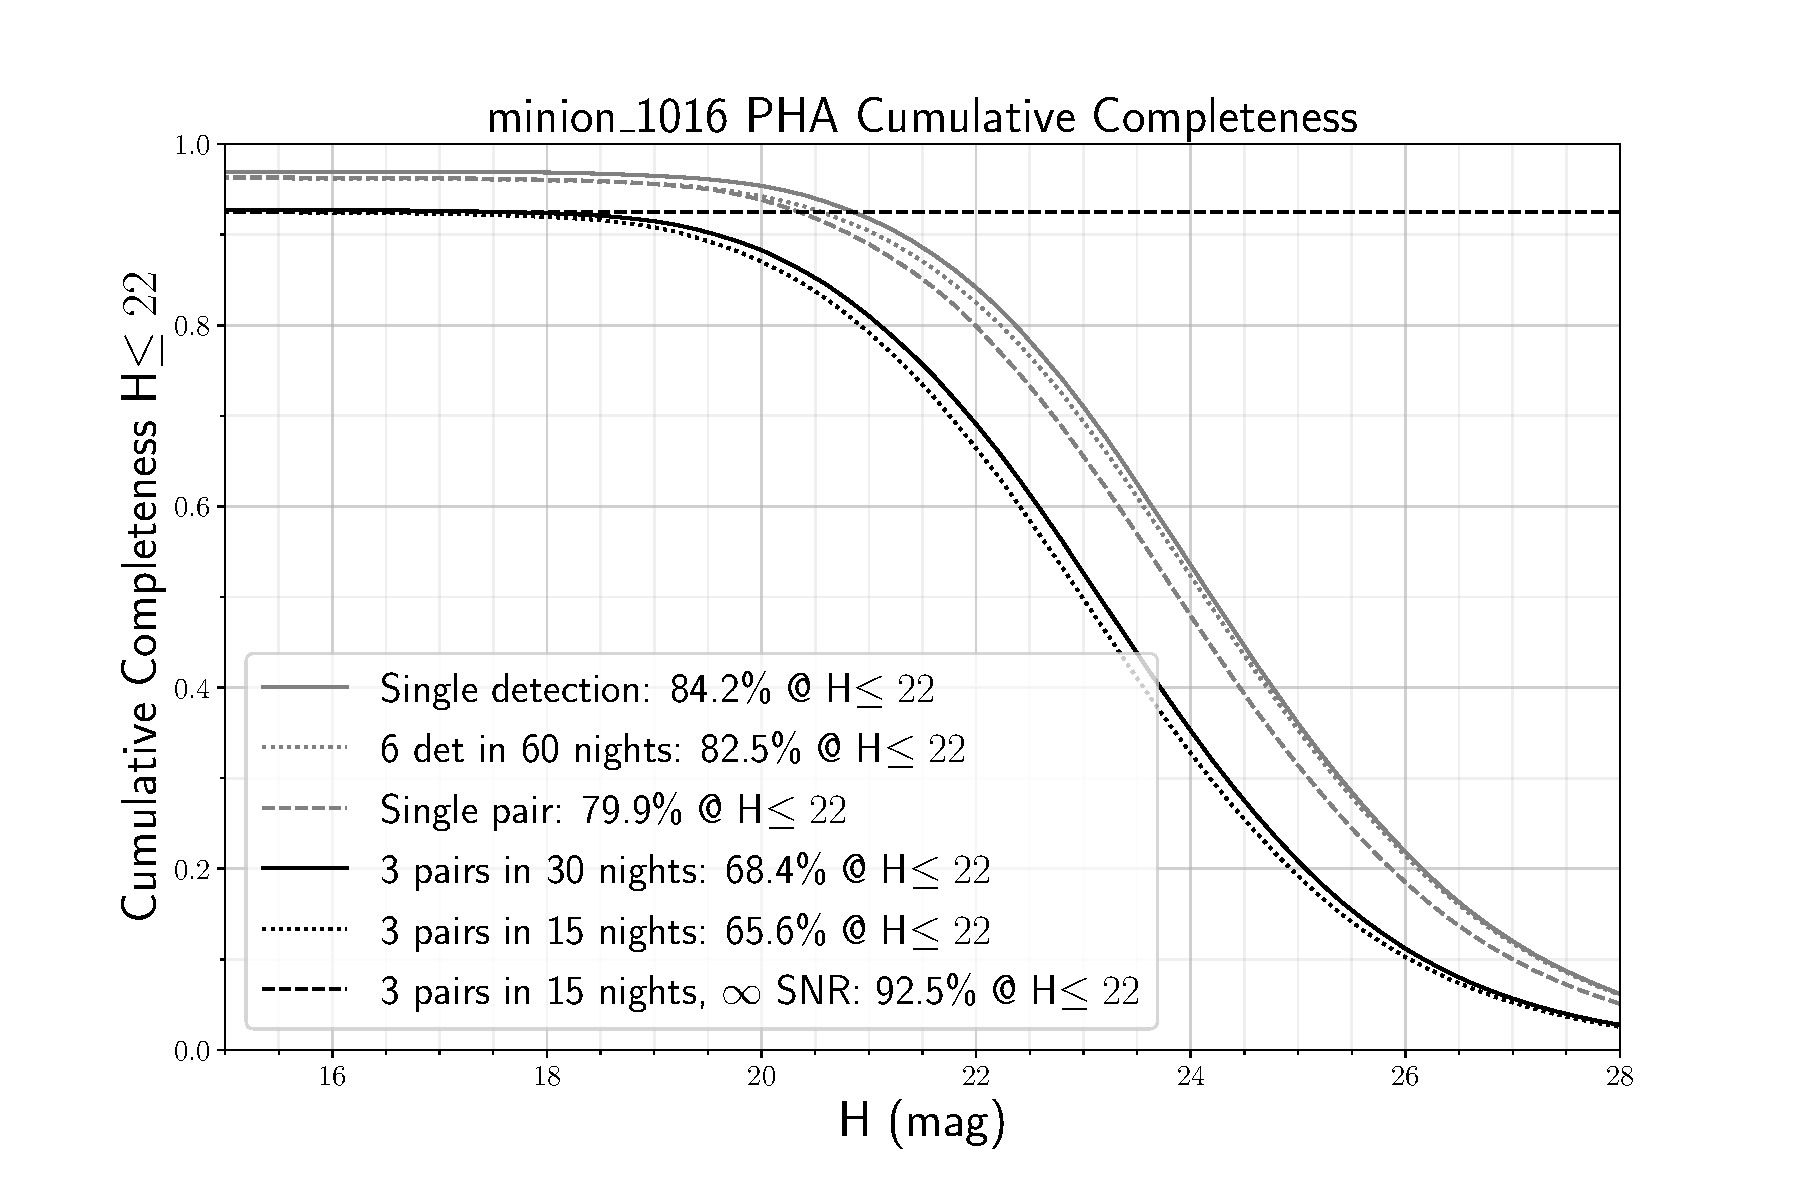
\includegraphics[width=0.99\textwidth]{figures/minion_1016_pha_More_Cumulative_Completeness}
\vskip -0.2in
\caption{The cumulative completeness for PHAs, as a function of absolute magnitude $H$, for the baseline
cadence minion\_1016, considering a variety of detection requirements. The completeness is below 100\% at the bright end (large size limit) because some objects have
synodic periods longer than the survey duration (and thus effectively ``hide'' behind the Sun), and also because some objects do not receive the required number of observations within the `window'. It is not due to the limited sensitivity of the LSST system, as can be seen by the ``3 pairs in 15 nights, $\infty$ SNR'' line, which shows the completeness expected when the discovery requirement is 3 nights with pairs of observations within a 15 night window but assuming an infinitely sensitive survey. The potential gains with better optimized scheduling (observing larger contiguous chunks of sky, for example), can be seen in the difference between the single pair of detections or 6 separate detections within 60 nights, vs. 3 pairs of detections in 15 or 30 nights (indicating potential gains of over 10\% in completeness for $H\le22$). \label{fig:more_completeness}}
\end{figure}

\subsubsection{Enhancing the Discovery Yields: Survey Strategy}

\begin{figure}[t!]
	\centering
	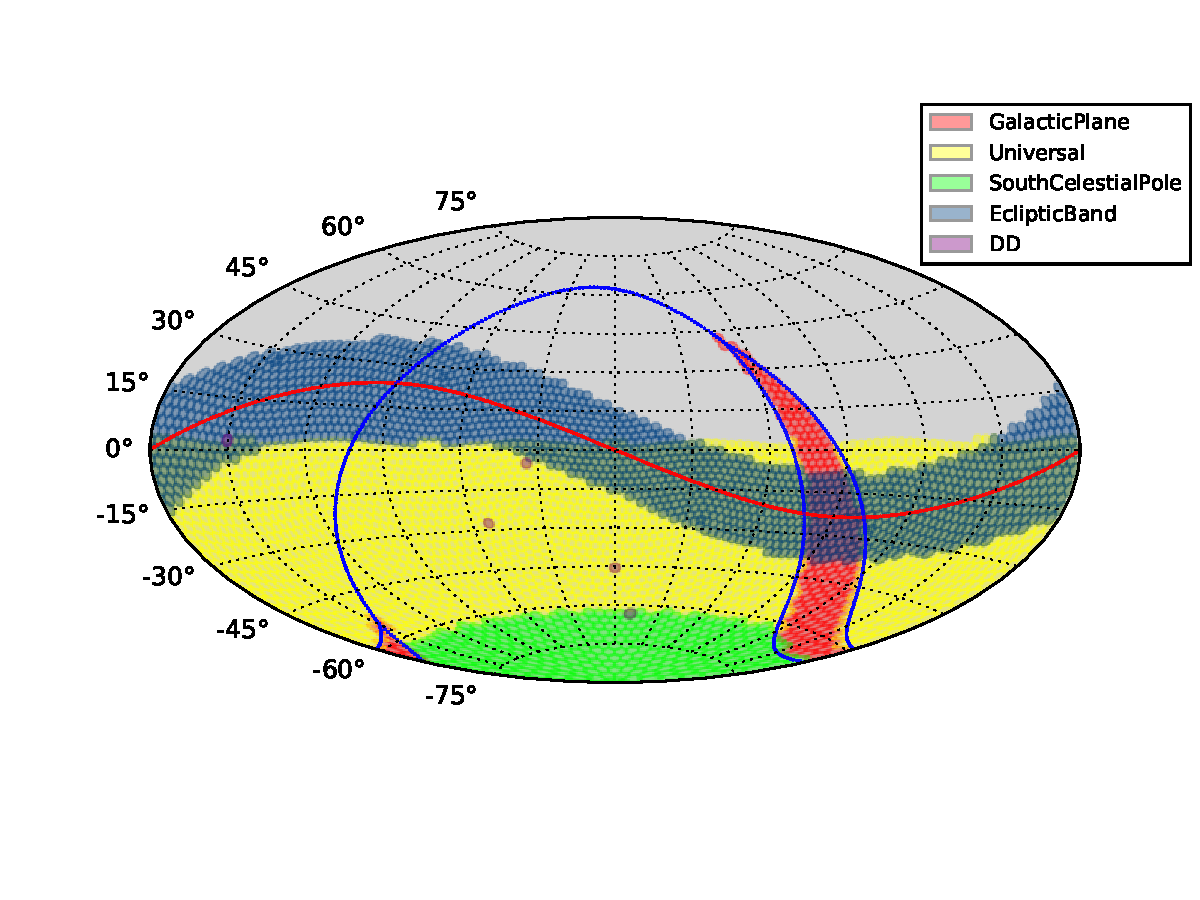
\includegraphics[width=0.49\textwidth]{figures/astro_lsst_01_1015_proposal_footprint}
	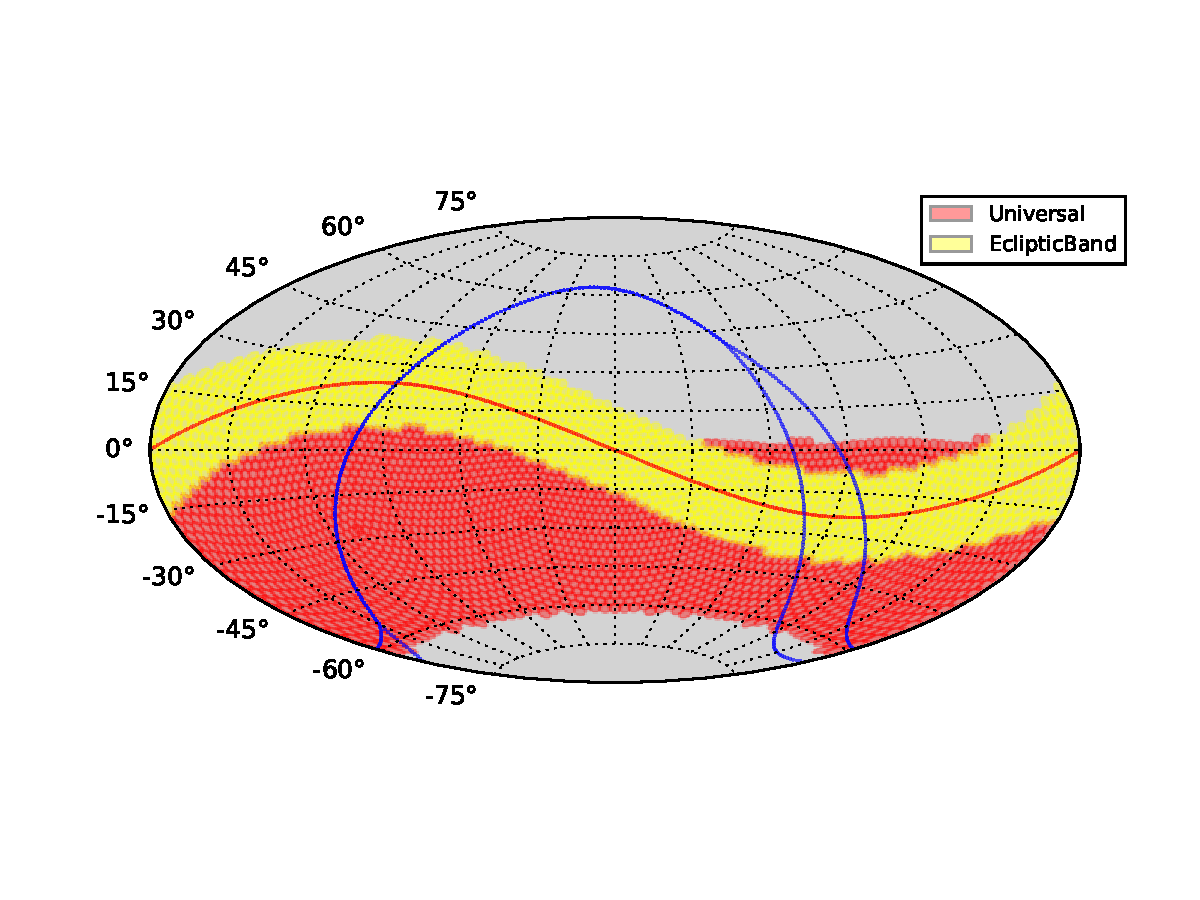
\includegraphics[width=0.49\textwidth]{figures/astro_lsst_01_1017_proposal_footprint}
	\vskip -0.5in
	\caption{The footprints of the proposals, including the Ecliptic Band proposal, used in the NEO-optimized simulated surveys astro\_lsst\_01\_1015 (the ``longer ecliptic visits'' survey, left) and astro\_lsst\_01\_1017 (the ``NEO-focused'' survey, right). The astro\_lsst\_01\_1017 survey only includes two proposals.
		\label{fig:neo_footprints}}
\end{figure}

We next look at modifying the survey strategy to increase LSST's NEO yields. We create a series of additional OpSim simulated surveys with parameters intended to improve the efficiency of discovering PHAs and increase the cumulative PHA completeness. These span the range from minor modifications to extreme changes that would jeopardize other LSST science goals. We consider the latter in order to assess what would be ultimate performance of an LSST-like system fully dedicated to NEO surveying.

The potential improvement in PHA discovery rates for modified survey cadences,
detailed in the rows of Table~\ref{tab:completeness}, is as follows:

\begin{itemize}
\item \textbf{Extra ecliptic visits:} By adding extra visits to the ecliptic spur (spending 24\% of survey time observing the NES proposal field, relative to 6\% in the baseline cadence), the increase in completeness over the LSST baseline is only about 0.5-1\%. This improvement comes at a cost to other science cases, as the main survey footprint (the WFD proposal) only receives 1,715,354 visits (82\%) of the number of visits in the reference run; the outcome of many science programs is roughly proportional to the number of visits.

\item \textbf{A 12-year survey:} By extending the baseline survey strategy by additional two years, we find an increase in completeness of 4\% over its completeness at the 10 year mark.

\item \textbf{Extra ecliptic visits, over 12 years:} We next look at the completeness of the ``extra ecliptic visits'' strategy, if extended to 12 years. We find it's better by $\sim 5$\% relative to the baseline.

\item \textbf{Longer visits in the ecliptic:} This strategy is visualized in the left panel of Figure~\ref{fig:neo_footprints}. The simulation requests longer, 60 second, visits in a band of $\pm 15^\circ$ around the ecliptic plane (the ``Ecliptic Band'' -- EB -- proposal).

The strategy reaches fainter limiting magnitudes, but the improvement due to longer exposures is counteracted by the fact that trailing losses are also increased. Similarly, the increase in the exposure time near the Ecliptic trades off against the revisit frequency reducing the number of opportunities for sets of observations that MOPS can successfully link. 

Because of that, this survey strategy show a slight {\em decrease} in completeness (percent level), relative to the baseline processed with the same software. Only if we assume the object detection pipelines can be modified to optimally detect trailed objects, a slightly higher PHA completeness level (~0.5\%) is achieved.

\item \textbf{NEO-focused survey:} This survey is visualized in the right panel of Figure~\ref{fig:neo_footprints}. It uses a limited filter set, discards other proposals, and uses longer exposures along the ecliptic. This strategy shows a slight increase in completeness ($\sim1-3$\%) relative to the baseline.
However, other LSST science programs would be jeopardized with this observing strategy because observations in the $uzy$ filters,
as well as special program observations would not be obtained.
\end{itemize}

To summarize, when altering the survey strategy the largest individual gain ($\sim$4\%) comes from simply extending the survey duration from 10 to 12 years. Other tested variants result in smaller marginal improvements, yet negatively affect other LSST science cases (most severely so in the case of the aggressive NEO-focused strategy).

\subsection{LSST in the Context of the Broader NEO Discovery System\label{sec:known}}

The completeness estimates presented above assumed that no objects are known prior to LSST survey or 
discovered by other resources during the LSST lifetime. When those contributions are taken into account, the completeness achieved by the entire system is significantly higher than what LSST alone can deliver.

%Evaluating the impact of existing and future resources in addition to LSST requires a model of how 
%specific NEOs and PHAs are discovered by other resources, in order to remove these objects
%from the list of objects discovered by LSST and properly account for overlap. 

We estimate the discoveries contributed by these previous, current, and future resources 
using a model similar to \citet{VeresChesley2017neo}: 
after generating ephemerides for the same populations of NEOs and PHAs as above, daily from 2000--2034 
(the end of the extended LSST surveys), we clone the objects over the same range of $H$ as 
used in the discovery metrics above. Each clone is considered potentially discovered if, while it is at
a solar elongation greater than 100 degrees, it becomes brighter a given apparent magnitude threshhold: 
this threshhold is $V=20$ from 2000-2005 (corresponding to the LINEAR era), $V=21$ from 2005-2015 
(representing Catalina and PanSTARRS1), $V=22$ from 2015 to the start of LSST in 2022, and then
$V=22.2$ after 2022.  In each of these periods, it is possible that even if the objects are bright enough, 
they would not be discovered simply due to sky coverage constraints of the telescopes; to 
this we add an efficiency factor that accounts for how likely any given detection on a given night is to be achieved. 
This factor is held constant until 2022, and then doubled (together with the increase in magnitude 
limit) to account for future improvements in NEO survey resources. We tune the efficiency factor to match
the historical rate of discoveries reported on the JPL NEO discovery page\footnote{See https://cneos.jpl.nasa.gov/stats/totals.html}.

With this model, at the start of LSST, we estimate the known NEO population with $H<22$ to be 43\% complete
and the PHA population with $H<22$ to be 54\% complete. Our NEO estimate is in good agreement with those
from \citet{VeresChesley2017neo} and \citet{GMS2016} who predict 42\% and 43\% completeness for NEOs, respectively.
In 2032, at the nominal end of LSST, our model predicts 72\% completeness for PHAs and 59\% completeness for NEOs, all without LSST. For NEOs, \citet{VeresChesley2017neo}
predicts a slightly higher value of 61\% while \citet{GMS2016} predicts a lower value of about 52\%. 
Given the uncertainty in the assumptions being made about the evolution of other surveys over a 17 year time period, this variance is understandable.

Combining these discoveries with those in the baseline cadence ({\it minion\_1016} with 15 day windows) 
gives us the expectation for our knowledge of the the post-LSST completeness of PHAs and NEOs. We find:
\begin{equation}
C_{\rm PHA, baseline + system}(H\le22) = 81\%
\end{equation}
and
\begin{equation}
C_{\rm NEO, baseline + system}(H\le22) = 73\%
\end{equation}.
In other words, the Earth-approaching asteroids discovered by the LSST will add $\sim 10$ percentage points to what the system would have discovered (given our model assumptions).

Combining these discoveries with those from the ``extra ecliptic visits'' strategy under a 30-day MOPS linking window, we find that including the LSST into the NEO discovery system boosts overall PHA completeness to 84\% over a 10-yr period, and 86\% if the survey is extended to 12 years. These results are summarized in Figure~\ref{fig:knownObj} and Table~\ref{tab:completeness2}.


\begin{deluxetable}{lcccccc}
\tablecaption{The cumulative completeness (in \%) for NEOs and PHAs with $H\le22$ for
the 10 year LSST baseline survey strategy, with a linking window ($N_w$) of 15 days,
compared with an extended 12-year survey with additional visits along the
Ecliptic using 30 day linking windows. The estimate of completeness achieved by other surveys
without LSST is given in ``No LSST'', the estimate of LSST discoveries alone is given in ``Only LSST'', 
and the combination of LSST plus the larger discovery effort is given in ``LSST + others''. 
\label{tab:completeness2}}
\tablehead{
& \multicolumn{3}{c}{10 year baseline, $N_w$=15}  &  \multicolumn{3}{c}{12 year ``extra ecliptic visits'', $N_w$=30}  \\
\cmidrule(r){2-4} \cmidrule(r){5-7}
Population  & No LSST &  Only LSST & LSST + others &  No LSST  & Only LSST & LSST + others
}
\startdata
    NEO & 59 & 61 & 73 & 61 & 69 & 77 \\
    PHA & 72 & 66 & 81 & 74 & 74 & 86 \\
\enddata
\end{deluxetable}



\begin{figure}[t!]
\centering
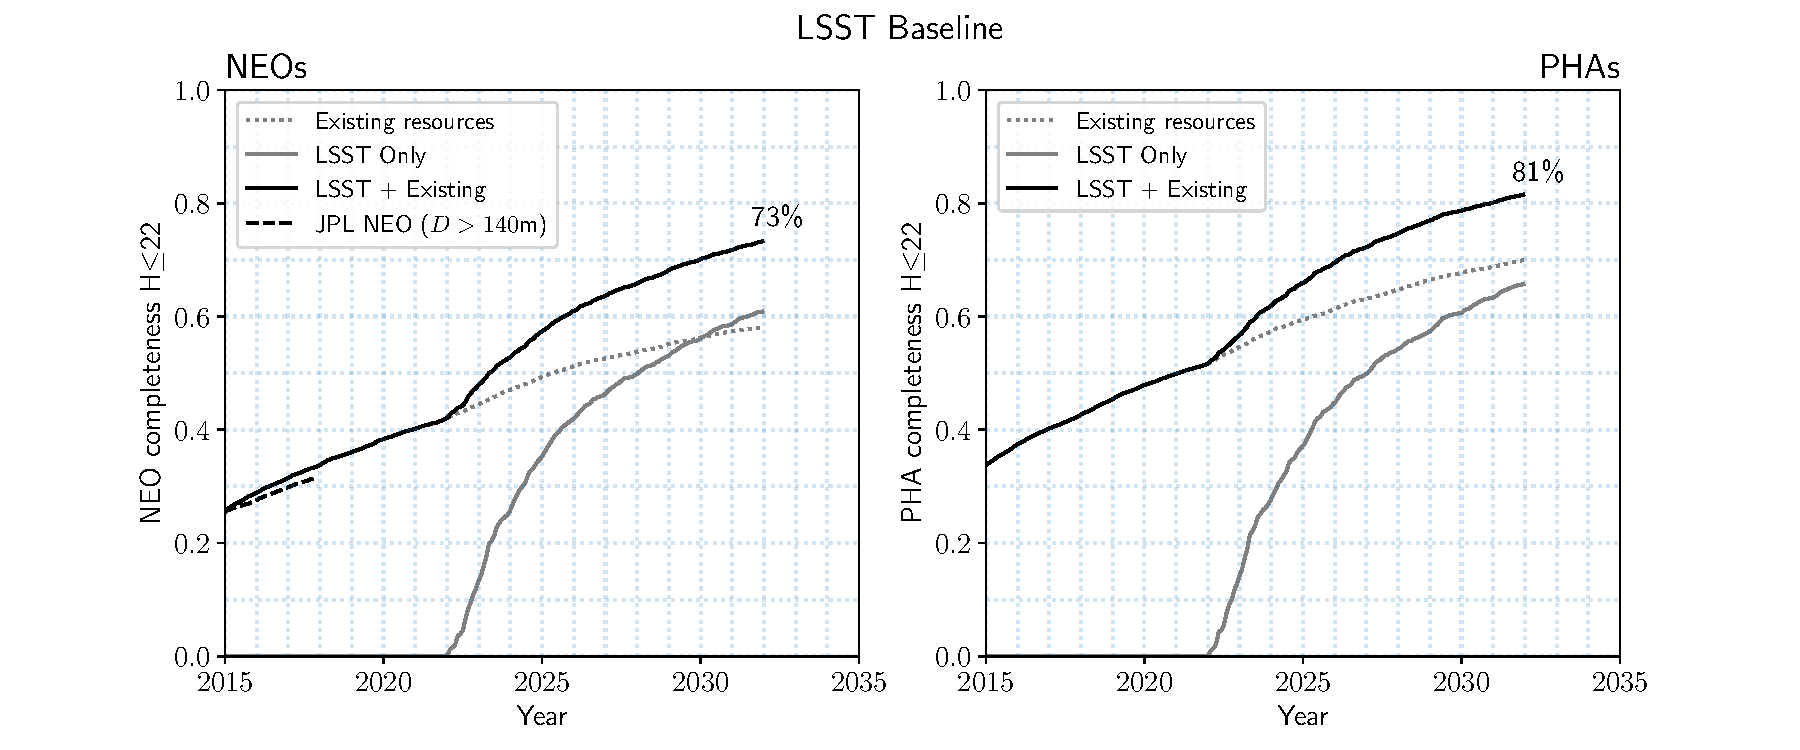
\includegraphics[width=0.99\textwidth]{figures/neo_pha_completeness_3in15_minion_1016.pdf} \\
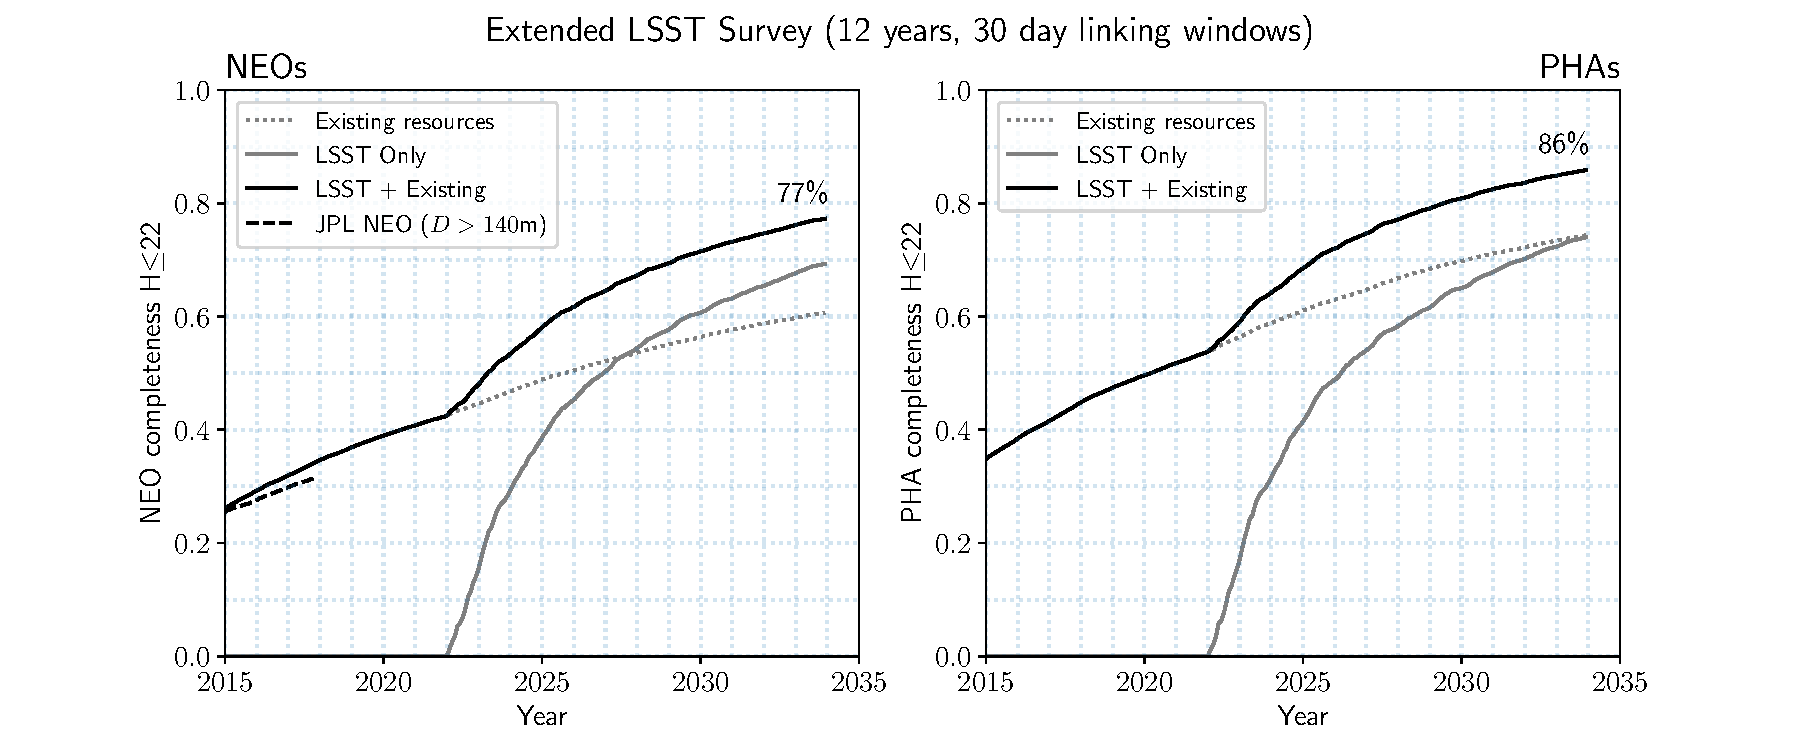
\includegraphics[width=0.99\textwidth]{figures/neo_pha_completeness_3in30_astro_lsst_01_1016.pdf}
\vskip -0.2in
\caption{The cumulative completeness for NEOs (left) and PHAs (right) with $H\le22$, as a function of
time, when known objects (gray solid lines) are taken (black solid lines) and not taken (dotted lines)
into  account (see also Table~\ref{tab:completeness2}). Discovery with existing and future resources 
is accounted for with a model that attempts to match expected limited magnitudes in each time period
and an efficiency factor that is tuned to match the rate of discoveries as reported by JPL (dashed line; see text for details). 
The top panel shows discoveries assuming the baseline LSST survey (10 year duration, with a 15 night tracklet linking window).
The bottom panel shows discoveries that could be achieved with the 12 year ``extra ecliptic visits'' LSST survey and a 30 night tracklet linking window.
\label{fig:knownObj}}
\end{figure}



\subsection{Systematic Effects due to Varying Modeling Assumptions \label{sec:syseff}}

As indicated by the above discussion, a number of systematic effects must be taken into account when
comparing different simulations of the same survey, as well as simulations of different surveys and observing
systems. Below we list the leading systematic effects in simulated completeness estimates:
\begin{enumerate}
\item Population choice - an NEO vs. PHA difference. We find the completeness is generally about $\sim$5\% higher for PHAs than for NEOs.
\item Orbital parameter distribution for the simulated asteroid population (e.g. the \citealt{Bottke2002} model
             vs. the Granvik, in prep., model). Varying populations contribute completeness uncertainty of about a few percent, based
             on simulations by \citet{VeresChesley2017neo}.
\item Different sample definitions: $H<22$ vs. $D>140$m; as shown by  \citet{2016AJ....152...79W} and \citealt{GMS2016},
          completeness increases by $\sim$5 percentage points (p.p.) when an $H$-based criterion is used instead of $D>140$m.
\item Variations of the ``discovery window'' (e.g., 3 nights with pairs of visits over $N_w$ nights: increasing
        $N_w$ from 15 to 30 increases completeness by about 3-5 p.p., while decreasing $N_w$ from 15 to 12 decreases 
        completeness by about 1-2 p.p. depending on the details of the survey cadence).
\item Uncertainties when predicting effective image depth (system throughput, background noise due to sky brightness, 
          variation of the detection efficiency with the signal-to-noise ratio, treatment of trailing losses). As a rule of thumb, for a survey that has a 
          completeness above 60\%, each additional 0.1 magnitude of depth for a given survey cadence increases the 
          completeness by another 1 p.p.
\item Uncertainties when predicting asteroid's apparent flux (albedo distribution, phase effects, photometric variability
          due to non-spherical shapes, color distributions); assuming an uncertainty of 0.2 mag in the effective
          limiting magnitude, the corresponding  systematic uncertainty in completeness is about 2 p.p.
\item Variations of the nominal detection threshold. If the detection threshold is changed from the
          signal-to-noise ratio of 5 or greater to 4 or greater, the completeness is boosted by $\sim$3~p.p.;
          the difference between the optimal detection using trailed profile and point-spread-function
          detection, which is negligible for LSST baseline exposure time of 30 seconds, would be worth $\sim$1.5~p.p.
          in completeness for visits with a doubled exposure time.
\item Sensitivity to details in sky coverage and cadence (e.g. nightly pairs of visits vs. quads of visits).
          Requiring quads instead of pairs of visits decreases completeness by 30\% using the baseline cadence;
          about half of that loss can be recovered using cadence simulations that request four visits per night.
\item The slope of the asteroid size distribution. Current measurement uncertainty of this parameter
          corresponds to a systematic uncertainty in completeness of about 2\%.
\item The impact of known objects. As discussed in \S\ref{sec:known}, we estimate that 54\% of PHAs with $H<22$ would be discovered
          by current survey assets by the start of LSST survey in 2022 (currently $\sim$36\%), and they would
          boost the final PHA completeness after a 10-year LSST baseline survey by 14~p.p. But different models and assumptions on the future development of the NEO system make this number uncertain to at least $\sim 3-5$~p.p.
\end{enumerate}

Given all these, it is unlikely that a meaningful quantitative comparison of different studies can be expected beyond a level of a few percent. The same is true of the accuracy of an estimate vs. actual realized performance. The exact magnitude of that uncertainty is difficult to estimate as the various effects don't add up coherently, aren't equally likely, with some being poorly constrained. Effects 1, 3, 4, 7, and 8 are a matter of definition/input. Adding all other effects in quadrature yields a notional ``error bar'' of $\sim 5$ percentage points, which we adopt here.

\subsection{Comparison to Other Works  \label{sec:other}}

Two recent works, \citet*[][hereafter GMS]{GMS2016} and \citet*[][hereafter VC]{VeresChesley2017neo}, 
have also evaluated the NEO completeness that could be achieved with a baseline LSST survey.
GMS reported a cumulative completeness for NEOs of 63\%, 62\% for PHAs,
while VC reported a cumulative completeness of 61.6\%  for NEOs and 64.9\% for PHAs, 
for a baseline survey with $N_w$ = 15 days. These can be compared with our estimates of 61\% for NEO completeness
and 66\% for PHA completeness.

All these results are consistent, given the understood systematic differences discussed in \S\ref{sec:syseff}. We identify three main reasons that contribute to the (small) differences:
\begin{enumerate}
\item The definition of the completeness limit: $H\le22$ or $D>140$m. By using an albedo distribution combined 
with a size distribution, GMS directly model the population larger than 140m rather than those with $H\le22$. 
Using $H\le22$ can lead to a increase in completeness on the order of 5\% \citep{2016AJ....152...79W, GMS2016}.
\item The realization of the LSST baseline survey, including the sky brightness model, system sensitivity model, and
delivered seeing distribution.  GMS used an older realization of the LSST baseline survey, {\it enigma\_1189}, which
had limiting magnitudes that were on average fainter by a few tenths of a magnitude than they are in 
{\it minion\_1016}, a more recent baseline survey with updated values for the system throughput and seeing. 
The decrease in limiting magnitudes in {\it minion\_1016} leads to a decrease in completeness of about 2\% compared
with GMS results.
\item Different realizations of the input populations. The major difference here is between NEO and PHA populations,
which leads to the difference in completeness in our results and the results from \citet{VeresChesley2017neo}.
However, small differences in the source of the input population can also lead to differences on the level of a few percent \citep{VeresChesley2017neo}. 
\end{enumerate}

Therefore, after accounting for different choices of simulation parameters 
we conclude the GMS and VC results for baseline NEO discovery efficiency are in excellent mutual agreement (within 1-2 \%), as well as in agreement with the analysis presented in this paper.
